\documentclass[dvipdfmx,uplatex]{jsarticle}

%% Packages
\usepackage{graphicx,color,hyperref}
\usepackage{algorithm}
\usepackage{algorithmic}
\usepackage{url}
\usepackage{lscape}
\usepackage{mathtools}
\usepackage{here}
\usepackage{amsmath,amssymb,amsfonts}
\usepackage{amsthm}
\usepackage{tikz}
\usepackage{tcolorbox}
\usepackage{pxjahyper}

%% Theorem Styles
\newtheorem{theorem}{定理}
\newtheorem{proposition}{命題}
\newtheorem{cor}{系}
\newtheorem{definition}{定義}
\newtheorem{problem}{問題}
\theoremstyle{remark}
\newtheorem{remark}{注意}
\newtheorem{requirement}{条件}

%% Environment (Colorful Box)
\newenvironment{simplebox}{
    \begin{tcolorbox}[
        fonttitle=\bfseries,
    ]
}{
    \end{tcolorbox}
}

\newenvironment{method}[1]{
    \begin{tcolorbox}[
        colframe=green!50!black,
        colback=green!50!black!10!white,
        colbacktitle=green!50!black!40!white,
        coltitle=black,
        fonttitle=\bfseries,
        title={#1}
    ]
}{
    \end{tcolorbox}
}

\newenvironment{experiment}[1]{
    \begin{tcolorbox}[
        colframe=violet,
        colback=violet!10!white,
        colbacktitle=violet!40!white,
        coltitle=black,
        fonttitle=\bfseries,
        title={#1}
    ]
}{
    \end{tcolorbox}
}

\newenvironment{kansou}{
    \begin{tcolorbox}[
        colframe=brown,
        colback=brown!10!white,
        colbacktitle=brown!40!white,
        coltitle=black,fonttitle=\bfseries
    ]
}{
    \end{tcolorbox}
}

%% Title
\title{ReAcTable: Enhancing ReAct for Table Question Answering}
\author{\empty}
\date{\empty}

%% Document body
\begin{document}
\maketitle

\begin{itemize}
    \item Link: \url{https://www.vldb.org/pvldb/vol17/p1981-zhang.pdf}
    \item Conference: VLDB2024
    \item Citation: \cite{ReAcTable}
    \item Arxiv: \url{https://arxiv.org/abs/2310.00815}
\end{itemize}

\section{概要}
\begin{simplebox}
\begin{itemize}
    \item Table Question Answering (TQA)においては自然言語でデータを分析するというタスクである、このタスクにReActの技法を用いることでその精度を向上させた。
    \item この手法をReAcTableと名付け、この手法はWikiTQベンチマークで2.1\%スコアを更新し、68\%の精度を達成する。
\end{itemize}
\end{simplebox}

\section{背景}
\begin{simplebox}
\begin{itemize}
    \item Chain Of Thought (CoT): LLMの推論過程を複数のステップに分け、モデルが単純化された問題を解くことで複雑な問題を解決する手法。
    \item ReAct: ReasoningとActionを行い、LLMが外部環境と対話しながら問題を解決する手法。推論、行動、その結果を観察してまた推論、、と繰り返すことで問題を解決する。
    \item Table Question Answering (TQA): 自然言語で表形式のデータに対する質問に答えるタスク。
\end{itemize}
\end{simplebox}

\section{手法}
\begin{method}{ReAcTable}
\begin{itemize}
    \item 概要
    \begin{itemize}
        \item 概要は図\ref{fig:overview}に示す
        \item 入力はテーブルと自然言語による質問
        \item それに対してLLMは(i)SQLクエリの生成、(ii)Pythonコードの生成、(iii)直接質問に答える、のいずれかの方法で応答を行う
        \item 上の応答でコードが実行された場合はその結果ももとにまた応答を行う、最終的に質問で答えた場合にはその答えを出力する
    \end{itemize}
    \item プロンプト
    \begin{itemize}
        \item プロンプトは前回の反復でのLLMの出力に基づいてインスタンス化されるプロンプトテンプレートを使用する。個のプロンプトには元のテーブル、ユーザの自然言語での質問、前回の反復でのLLMの出力が含まれる。
    \end{itemize}
    \item 外部コード実行器の使用
    \begin{itemize}
        \item コード実行を行うがその際の例外処理を行う。
        \item SQL例外: SQLクエリの実行に失敗した場合は、その対象のテーブルの前の反復で生成されたテーブルにクエリを実行するというリトライ処理を行う。
        \item Python例外: Pythonコードでモジュールがない旨のエラーが発生する場合はそのモジュールを動的にインストールして実行する。 
    \end{itemize}
    \item どのように次のステップを選ぶかについて(図\ref{fig:voting}参照)
    \begin{itemize}
        \item マジョリティ投票: 最後の答えを出力するまでLLMに反復させ、その多数決を行う
        \item ツリー探索: 各反復でいくつかの異なる応答を生成し、それらの応答をツリー構造で探索することで、最終的な答えを導き出す。
        \item 実行ベース投票: 各反復で生成されたSQLクエリやPythonコードを実行し、その結果に基づいて次のステップを一つ選択する。
    \end{itemize}
\end{itemize}
\end{method}

\begin{figure}
    \centering
    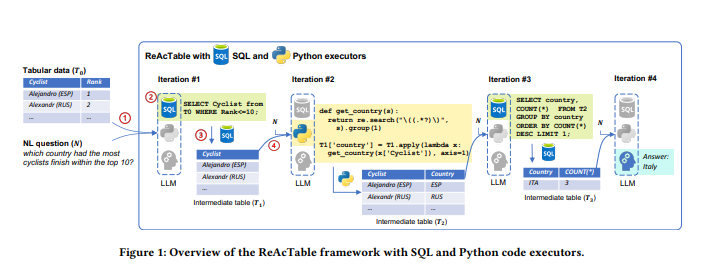
\includegraphics[width=0.5\textwidth]{img/ReAcTable/overview.png}
    \caption{ReAcTableの全体概要}
    \label{fig:overview}
\end{figure}

\begin{figure}
    \centering
    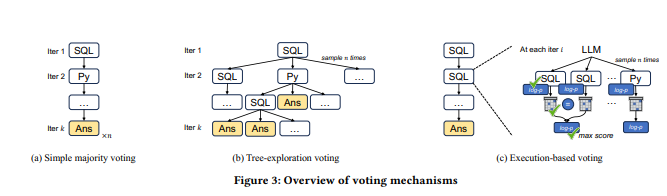
\includegraphics[width=0.5\textwidth]{img/ReAcTable/voting.png}
    \caption{ReAcTableの投票メカニズム}
    \label{fig:voting}
\end{figure}

\section{実験結果}
\begin{experiment}{実験手法}
\begin{itemize}
    \item ベンチマーク: WikiTQ, TabFact, FeTaQAの3つを使用する
    \item ベースライン: 学習を必要とする手法(e.g. MAPO)、学習を必要としない手法(e.g. Binder, Dater)の両方を利用する
    \item ReAcTableの設定: 3つの投票法の有無に応じたReAcTableの性能を比較する.
    \item 評価指標: 出力がタプルである場合はその一致率、自然言語である場合はROUGE-N, ROUGE-L指標を用いる
\end{itemize}
\end{experiment}

\begin{experiment}{実験結果}
\begin{itemize}
    \item 結果A
\end{itemize}
\end{experiment}

\begin{experiment}{ReAcTableの分析}
\begin{itemize}
    \item 中間テーブルの効果
    \item 反復回数の効果
    \item Python実行器の効果
    \item 異なる多数決方式の効果
    \item レイテンシ
\end{itemize}
\end{experiment}

\section{感想}
\begin{kansou}
\begin{itemize}
  \item この手法はテーブルに入っているデータに関する質問について一回のSQL生成で答えを出すのではなく、複数回SQL生成を繰り返すことで、より正確な答えを導き出すことができるのだなと思った。一回ではなく何回か反復させることがほかの研究との違いだと思う。
  \item まだ単一のテーブルに対する質問しか答えていなくて、これから複数のテーブルに拡張したときにこの手法がどのような効果を発揮するのかが気になる。
\end{itemize}
\end{kansou}

\bibliographystyle{jplain}
\bibliography{template.bib}

\end{document}